\section{Data Acquisition}
\label{sec:chap_slam_data_acquisition}

In the following section, we first describe the robotic platform and sensors used to gather our place recognition dataset. We then describe in more details the dataset acquisition procedure and the resulting data.


\subsection{Robotic platform}
\label{ssec:chap_slam_platform}

The Husky A200 is a medium size (990 x 670 x 390 \SI{28}{\milli\meter}) \gls{ugv} developed by Clearpath Robotics~\cite{ClearpathWeb}. It is a rugged robot designed for all terrain conditions, therefore well suited for our experiments in forest. It uses a differential-drive skid steer allowing easy control and in place turns for our data acquisition. It has a maximum speed of \SI{1}{\meter\per\second}, but we generally acquire data at lower speed, which minimizes odometry and range data errors. This platform, with a maximum payload capability of \SI{75}{\kilo\gram}, can easily carry all sensors used for our experiments. The platform is shown in figure~\ref{fig:chap_slam_husky} and more details about the available devices are presented in table~\ref{tab:husky_devices} show a list of devices available on the platform and the use we make of them.

The on-board computer is an essential element of our experiments, as it connects all devices, acts as a control interface for the robot and stores acquired data. The computer does not provide a \gls{gui}, but it is connected to the gateway that broadcasts a WiFi network, allowing \gls{ssh} communication. The platform is also equipped with a wireless gamepad, which allows controlling the movements of the latter. Point clouds acquisition is possible using either the SICK LMS151 or the Velodyne HDL-32E. The selected sensor is mounted on the \gls{ptu}, which remains fixed for the Velodyne, but is rotated with the SICK to merge multiple \gls{2d} scans into a single \gls{3d} point cloud.

For our place recognition research, we mainly use the wheel encoder along with the \gls{imu} for odometry estimation. 

\begin{figure}
    \centering
    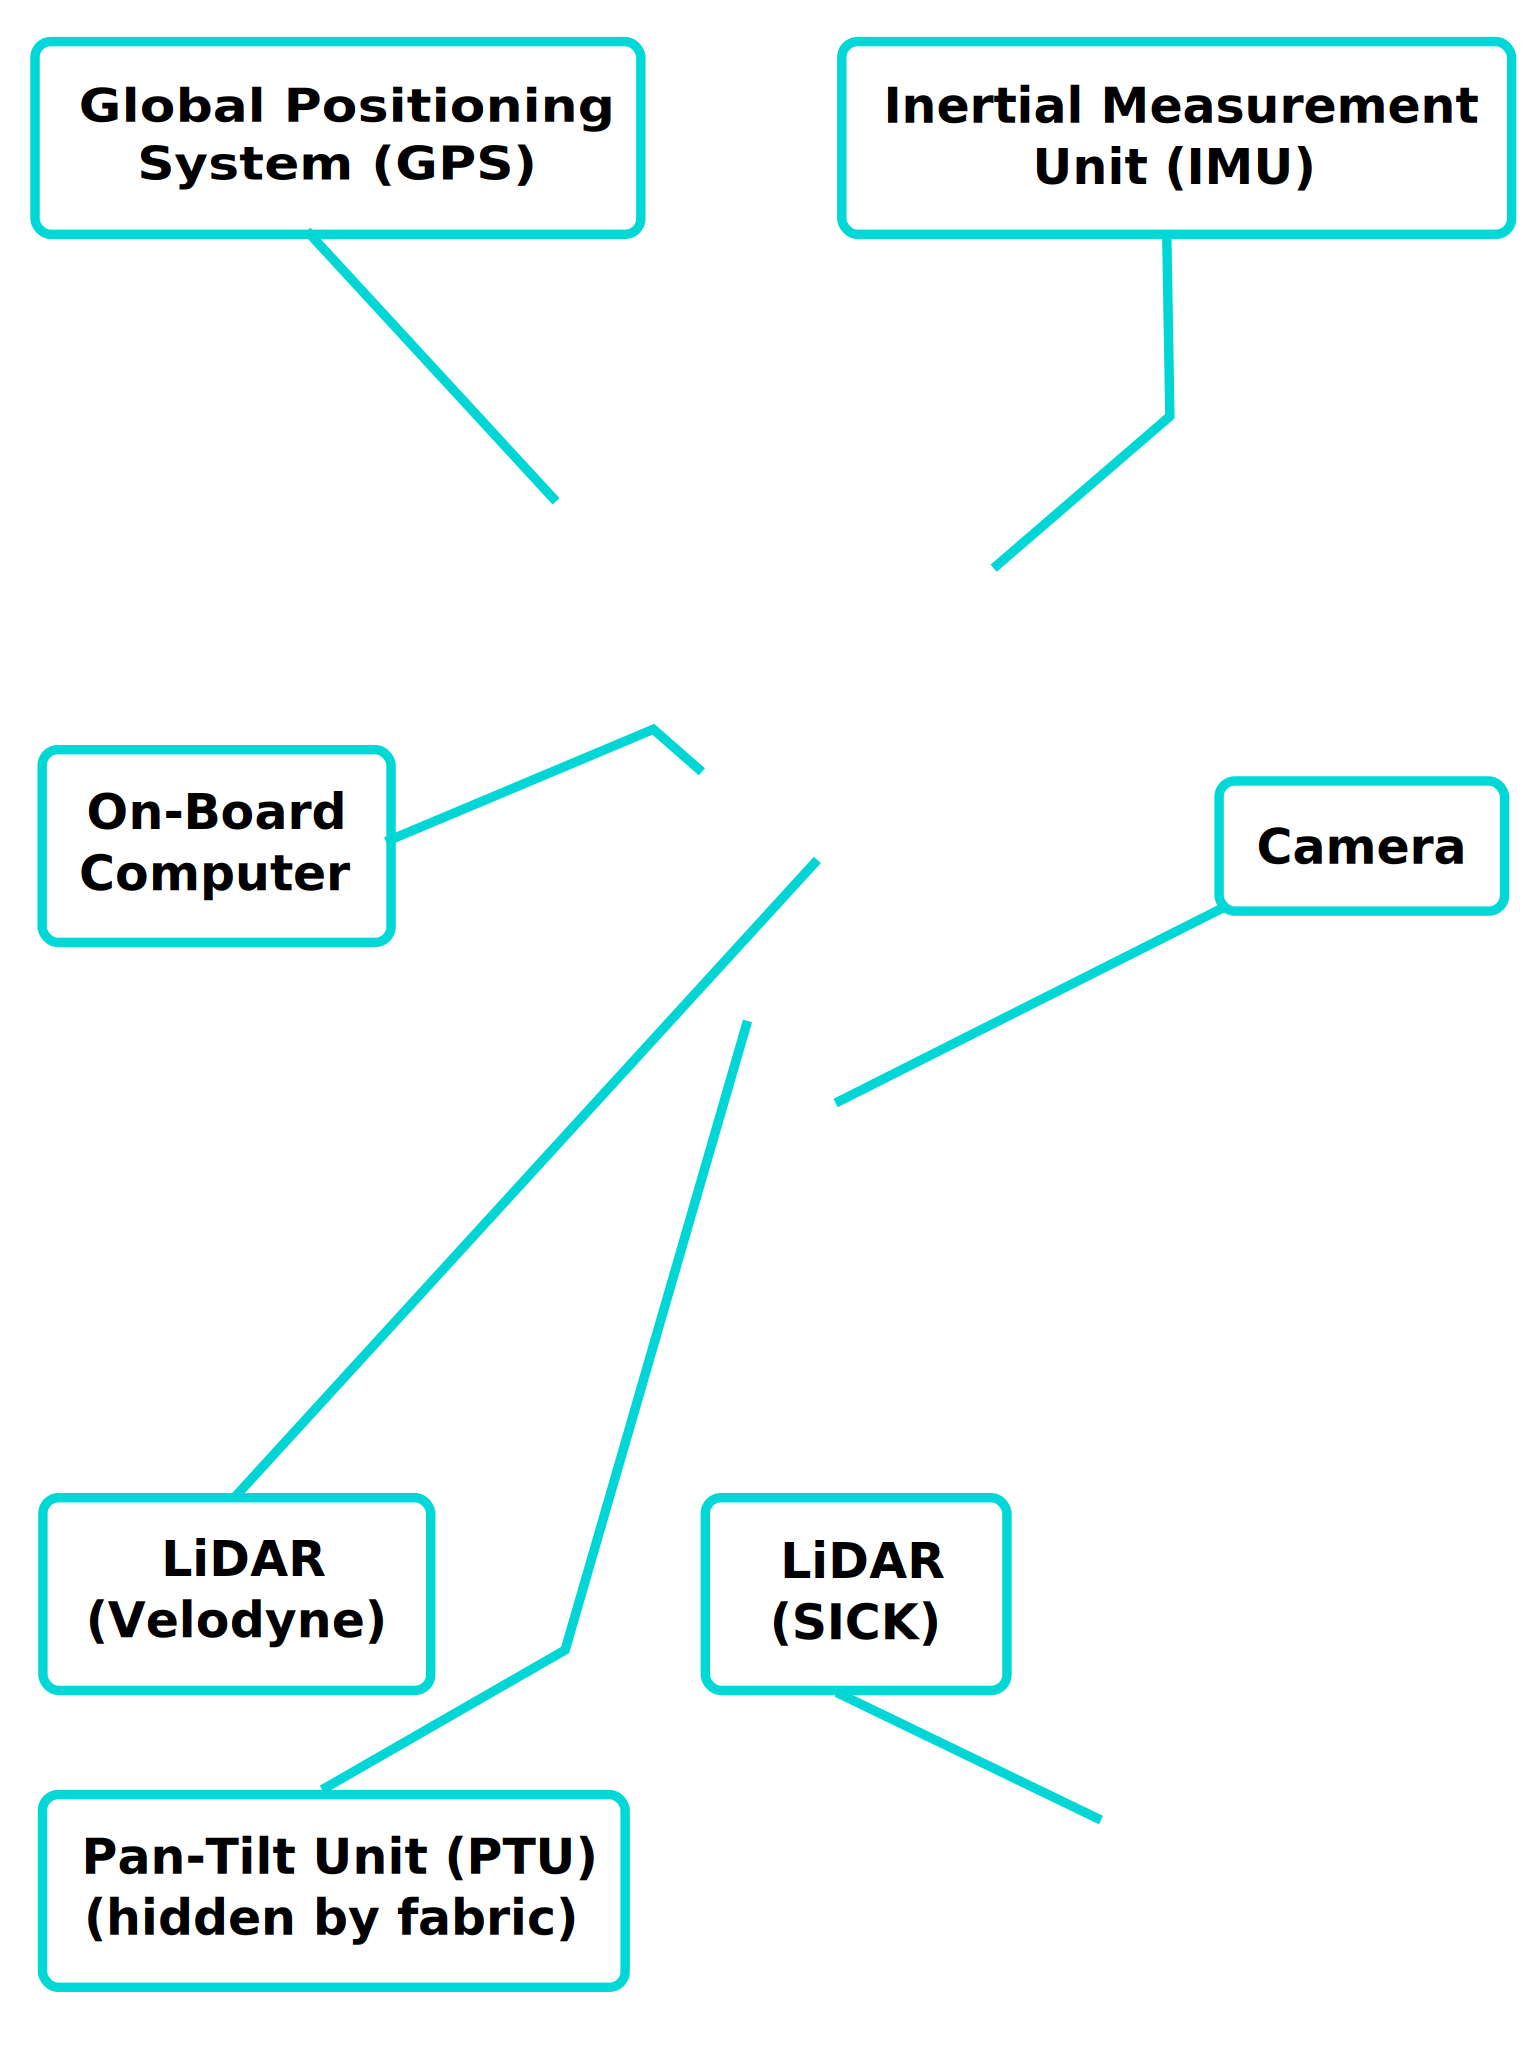
\includegraphics[width=0.98\linewidth]{img/chap_slam/husky_labelled.png}
    \caption{The robotic platform (Husky A200) and the devices used for data acquisition. The SICK \gls{lidar} is not mounted, but is shown on the bottom right corner of the figure. Note that the \gls{ptu} is hidden by fabric and the on-board computer is mostly occluded by the Velodyne \gls{lidar}.}
    \label{fig:chap_slam_husky}
\end{figure}

\begin{table}[h]
    \centering
    \begin{tabular}{|c|c|c|c|}
        \hline
        \textbf{Device} & \textbf{Manufacturer}       & \textbf{Model}  & \textbf{Use}                          \\ \hline
        Computer        & --                          & --              & Data acquisition/synchronisation      \\ \hline
        Gateway         & --                          & --              & Network and Wi-Fi communication       \\ \hline
        Gamepad         & Logitech                    & F710            & Remote control of the robot movements \\ \hline
        \gls{lidar}     & Velodyne                    & HDL-32E         & Point cloud acquisition               \\ \hline
        \gls{lidar}     & SICK                        & LMS151          & Point cloud acquisition               \\ \hline
        \gls{ptu}       & FLIR Motion Control Systems & D46-17          & Rotate the SICK \gls{lidar}           \\ \hline
        \gls{imu}       & ChRobotics                  & UM6             & Odometry                              \\ \hline
        %Wheel encoder   & Keep ?                      &                 & Odometry                             \\ \hline
        Camera          & Axis                        & M1013           & Visual reference                      \\ \hline
        \gls{gps}       & NovAtel                     & SMART6          & Not used                              \\ \hline
    \end{tabular}
    \caption{\label{tab:husky_devices} Set of devices available on the Husky A200 and their use in our experiments. Note that both \gls{lidar}s are not mounted at the same time,}
    \label{tab:husky_sensors}
\end{table}

\subsection{Dataset}
\begin{figure}[htpb]
    \centering
    \subfloat[]{\label{fig:path_overview}}{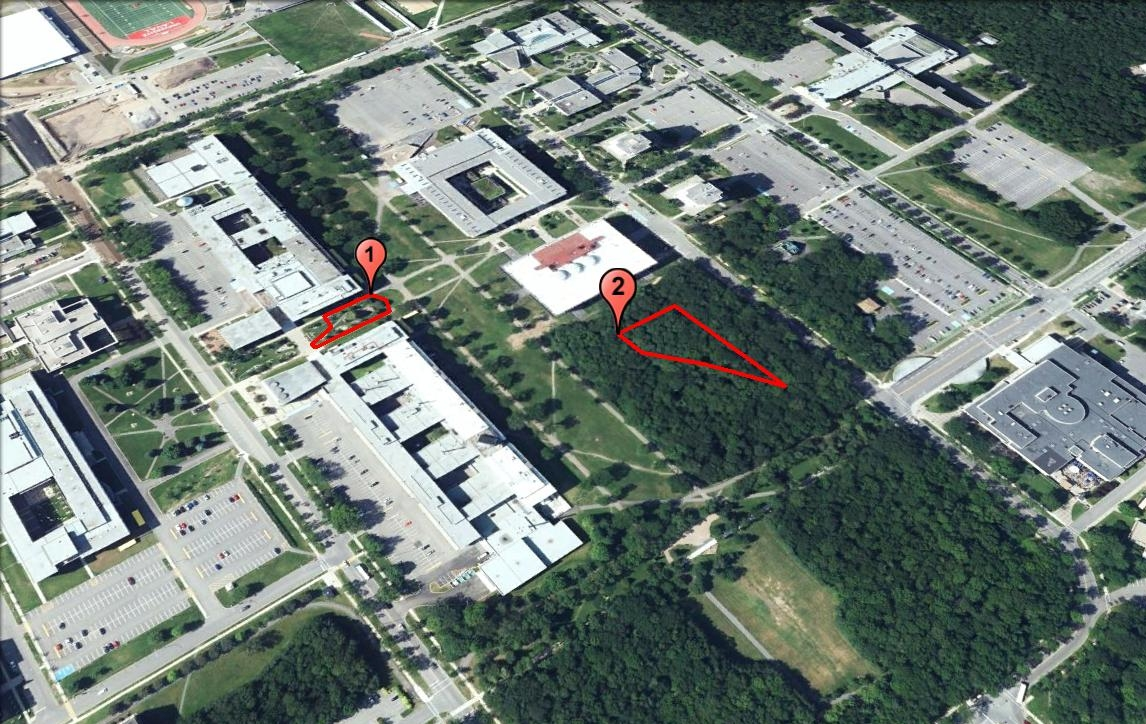
\includegraphics[width=0.97\linewidth]{img/chap_slam/paths.jpg}}\\ \vspace{3mm}
    \subfloat[]{\label{fig:path_building}}{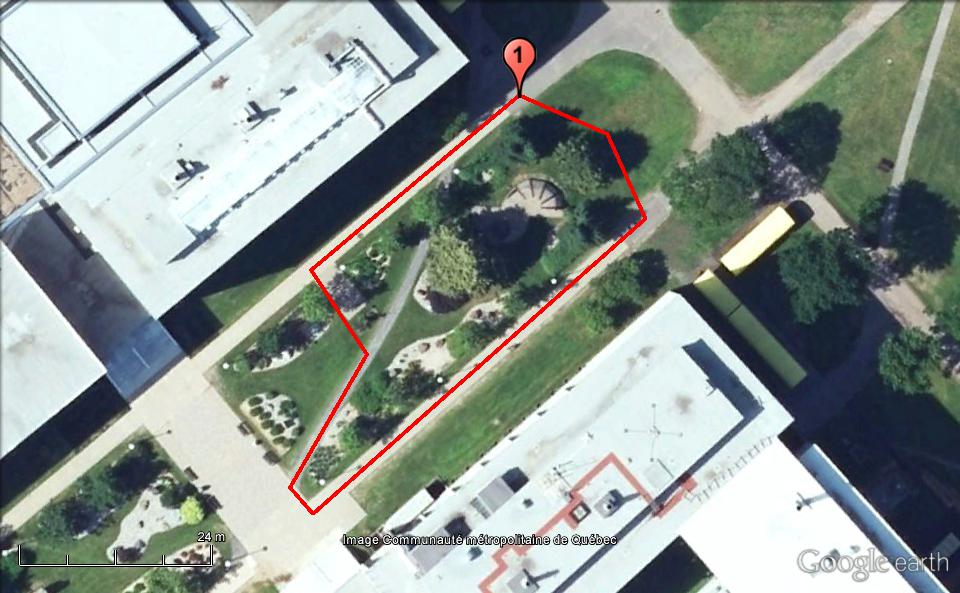
\includegraphics[width=0.413\linewidth]{img/chap_slam/path_building.jpg}} \hspace{2mm}
    \subfloat[]{\label{fig:path_forest}}{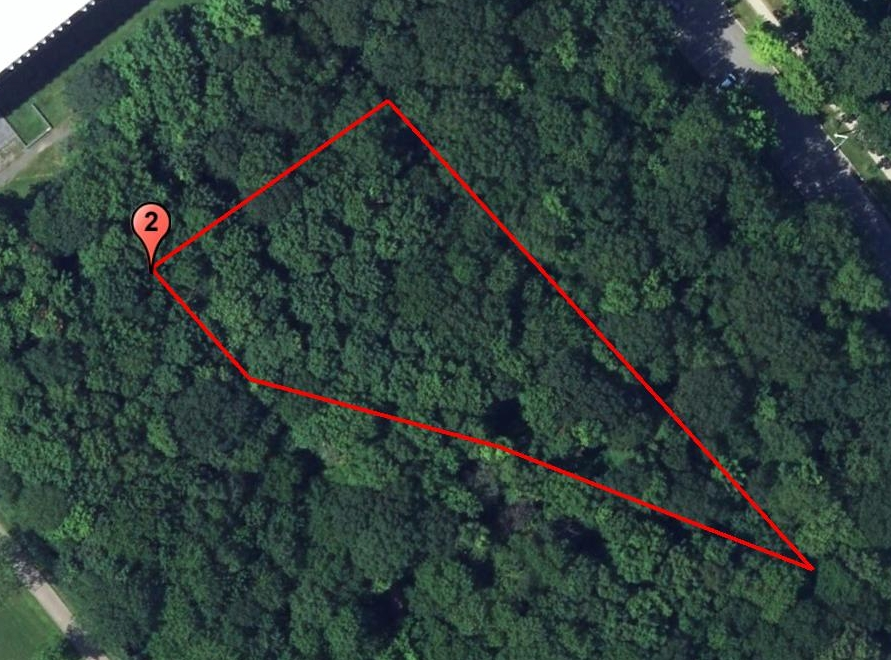
\includegraphics[width=0.529\linewidth]{img/chap_slam/path_forest.jpg}}
    \caption{\protect\subref{fig:path_overview} Partial aerial view of the Laval University campus including the two approximate paths followed by the robot for data acquisition. \protect\subref{fig:path_building} Zoomed view of the path followed (counterclockwise from tag 1) in a structured environment. The length of this path is approximately \SI{00}{\meter}. \protect\subref{fig:path_forest} Zoomed view of the path followed (clockwise from tag 2) to create the forest dataset. The length of this path is approximately \SI{280}{\meter}. Images source: Google Earth, (2015)}
    \label{fig:chap_slam_path}
\end{figure}


\subsection{Dataset description}
\label{ssec:chap_slam_platform}

\begin{itemize}
    \item Communication to onboard computer via ssh.
    \item There run nodes and record data (data synchronization).
    \item All data is post-processed (semi important)
    \item Describe environment for the 2 datasets (mainly flat, bulding, structure with table chair\dots. pedestrian road and offroad)
    \item Building vs forest (with SICK)
    \item SICK LMS151 vs velodyne (only in forest, angles/density, show point clouds side by side in a figure.)
    \item Give the acquisition date
    \item Talk about the correction using ICP
\end{itemize}
